%%%%%%%%%%%%%%%%%%%%%%%%%%%%%%%%%%%%%%%%%%%%%%%%%%%%%%%%%%%%%%%%%%%%%
% LaTeX Template: Project Titlepage Modified (v 0.1) by rcx
%
% Original Source: http://www.howtotex.com
% Date: February 2014
% 
% This is a title page template which be used for articles & reports.
% 
% This is the modified version of the original Latex template from
% aforementioned website.
% 
%%%%%%%%%%%%%%%%%%%%%%%%%%%%%%%%%%%%%%%%%%%%%%%%%%%%%%%%%%%%%%%%%%%%%%

\documentclass[11pt,a4paper]{article}
\usepackage[T1]{fontenc}
\AtBeginDocument{\usefont{\encodingdefault}{phv}{m}{n}}
\usepackage{helvet}
\usepackage{fullpage}
\usepackage[table,xcdraw]{xcolor}
\usepackage{fancyhdr}
\pagestyle{fancy}
\lhead{}
\setlength{\headsep}{0.3in}
\setlength\parindent{0pt}
\setlength{\parskip}{1em}
\usepackage[english]{babel}
\usepackage{amsmath}
\usepackage{siunitx}
\usepackage{graphicx}
\usepackage[colorinlistoftodos]{todonotes}
\usepackage{subfig}
%\usepackage{subcaption}
\usepackage[export]{adjustbox}[2011/08/13]
\usepackage[nottoc,numbib]{tocbibind}
\usepackage{float}
\usepackage{eurosym}
\usepackage{gensymb}
\usepackage{wrapfig}
\usepackage{multirow}
\usepackage[toc,page]{appendix}
\usepackage{hyperref}
\usepackage[all]{hypcap}
\usepackage[intoc]{nomencl}
\makenomenclature
 \usepackage{etoolbox}
\renewcommand\nomgroup[1]{%
  \item[\bfseries
  \ifstrequal{#1}{S}{Symbols}{%
  \ifstrequal{#1}{A}{Abbreviations}{%
  \ifstrequal{#1}{N}{Subscripts}{}}}%
  ]}
  \renewcommand{\nomname}{List of Abbreviations and Symbols}
%
\lhead{{\small Team 2R I. Zaman}}
%
\chead{{\small Weight and Balance, Stability \& Control}}
%
 \rhead{
\includegraphics[height=5mm]{Logo.png}}
%
\cfoot{\thepage}
\renewcommand{\headrulewidth}{1pt}
\usepackage[margin=2cm]{geometry}
\usepackage{titlesec}
\titlespacing{\section}{0pt}{5pt}{4pt}
\titlespacing{\subsection}{0pt}{5pt}{4pt}
\titlespacing{\subsubsection}{0pt}{5pt}{4pt}
\def\therefore{{\tiny$\bullet$}\kern-0.2ex\raisebox{1ex}{\tiny$\bullet$}\kern-0.2ex{\tiny$\bullet$}}
%-------------------------------------------------------------------------------
% TITLE PAGE
%-------------------------------------------------------------------------------

\begin{document}
\begin{titlepage}

\begin{figure}[H]
\minipage{0.32\textwidth}
  
\includegraphics[width=.75\linewidth]{University_of_Bristol_logo.png}
  \endminipage\hfill
  \minipage{0.32\textwidth}
  \centering
   % 
\includegraphics[width=.75\linewidth]{Logo.png}
    \endminipage\hfill
    \minipage{0.32\textwidth}%
    \hspace{12mm}
      \includegraphics[width=.75\linewidth]{Aero_logo.png}
      \endminipage
      \end{figure}

\center 
\vspace{20mm}
\hrule
%\textsc{\Large \textbf{Aerospace Vehicle Design \& System Integration 4 \\ \vspace{2mm} Final Engineering Definition Report}}

{\Large  \textbf{Weight and Balance, Stability \& Control \\ \vspace{2mm}
for an Electric Urban Air Vehicle (Skypass)}}
\vspace{10mm}
%\hrule

\textsc{\textbf{Ismaeel Zaman}} \\
\textsc{\textbf{(Team 2R)}}\\
\vspace{10mm}
\textsc{\textbf{Academic Advisor:} Professor Nick Lieven} \\
\textsc{\textbf{Postgraduate Mentor:} Harry Felton}
\\[0.5cm]

\vspace{24pt}
\textsc{\large Dated: January 2020} 
\vspace{6pt}

\hrule
\vspace{10mm}

% -----------------------------
%            ABSTRACT
% -----------------------------
%\textbf{Abstract:}
\abstract{Mass distribution and empennage are key issues when designing a balanced and stable rotary winged aircraft. The final positioning of component masses achieved a favourable CG envelope lying within 10.5cm of the rotor shaft under various payload configurations. The moments of inertia were calculated and fed into the design of the empennage. In the interests of passenger comfort, the absolute values of fuselage pitch at hover and cruise were kept as close to zero as possible whilst the resulting flapping angles of the rotors were minimised to reduce power consumption. This was achieved by specifying a particular shaft tilt and horizontal stabiliser configuration. The effect of each of these on the resulting flapping and pitch angles in both cruise and hover was analysed and an optimum combination found heuristically. The design specifies the rotor shaft tilt and the desired moment of the horizontal stabiliser. The aircraft is of a coaxial rotor design which does not require a vertical stabiliser or tail rotor. However, to improve passenger comfort and efficiency, a vertical stabiliser was dynamically modelled and a controlled rudder added to dampen oscillating yaw disturbances. The final specification provides a balance between passenger comfort and efficiency.}

%salaam
\begin{figure}[H]
    \centering
        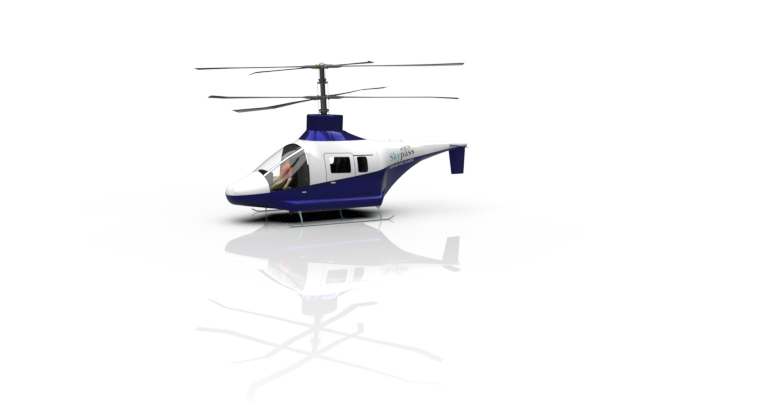
\includegraphics[width=0.5\textwidth]{High_res_2.png}
        \end{figure}
\hrule


\vfill
\end{titlepage}
\newpage
\setcounter{page}{1}
\pagenumbering{roman}
\tableofcontents
%\thispagestyle{empty}
\newpage
\listoftables
\newpage
\listoffigures
\newpage
% --------------------------
% Nomenclature 
% -------------------------
    \nomenclature[A]{CG}{Centre of Gravity}
    \nomenclature[A]{MTOW}{Max Take-off Weight}
    \nomenclature[A]{AUW}{All Up  Weight}
    \nomenclature[A]{MZFW}{Max Zero Fuel Weight}
     \nomenclature[A]{OWE}{Operational Weight Empty}
      \nomenclature[A]{NACA}{National Advisory Committee for Aeronautics}
    \nomenclature[S]{$I_{CG}$}{Second moment of inertia about CG, subscript refers to axis}
    \nomenclature[S]{W,mg}{Aircraft weight}
    \nomenclature[S]{M}{Moment, subscript refers to the part that generates the moment }
    \nomenclature[S]{L}{Lift force, subscript refers to lift generating part}
    \nomenclature[S]{$L_t$}{Tail Lift force (+downwards)}
    \nomenclature[S]{T}{Rotor total thrust}
    \nomenclature[S]{$\gamma$}{Rotor shaft tilt (- is tilt forward)}
    \nomenclature[S]{$\theta$}{Pitch Angle relative to free-stream (+ is nose-up), refer to subscript}
    \nomenclature[S]{$a_{1s}$}{Longitudinal Rotor flapping angle, (+forward disc tilt)}
    \nomenclature[S]{D}{Drag force, subscript refers to part, subsubscript may refer to direction}
    \nomenclature[S]{$h$}{Height of part above CG, subscript for part}
    \nomenclature[S]{l}{longitudinal distance of part from CG, subscript for part}
    \nomenclature[S]{S}{Surface area, subscript for part}
    \nomenclature[S]{$\rho$}{Air density}
       \nomenclature[S]{V}{Velocity}
          \nomenclature[S]{$C_{l_\alpha}$}{Lift curve slope}
             \nomenclature[S]{$C_{d_\alpha}$}{Drag curve slope}
             \nomenclature[S]{$\phi_t$}{Horizontal Tail setting angle}
             \nomenclature[S]{$\Omega$}{Rotor angular speed}
             \nomenclature[S]{$R$}{Rotor radius}
             \nomenclature[S]{$m_b$}{Mass of blade}
             \nomenclature[S]{$e$}{Blade Hinge offset}
             \nomenclature[S]{$b$}{Number of blades}
              \nomenclature[N]{$r$}{Rotor} 
              \nomenclature[N]{$h$}{Horizontal Stabiliser}
              \nomenclature[N]{$t$}{Horizontal Stabiliser}
              \nomenclature[N]{$v$}{Vertical Stabiliser}
              \nomenclature[N]{$tp$}{Vertical Static Fin}
              \nomenclature[N]{$R$}{Rudder}
              \nomenclature[N]{$f$}{Fuselage}

 
\printnomenclature
\newpage
\setcounter{page}{1}
\pagenumbering{arabic}
%\setcounter{page}{1}
%-------------------------------------------------------------------------------
% Section title formatting
%\sectionfont{\scshape}
%-------------------------------------------------------------------------------

%-------------------------------------------------------------------------------
% INTRODUCTION
%-------------------------------------------------------------------------------

\section{Introduction}
Helicopters can provide a fast point-point capability between locations within a limited range with a potential for direct access to urban areas. However, a cost effective and environmentally friendly means has been elusive. With recent developments in electrical power drives and batteries the potential for such transportation is increasing, with multiple companies such as Lilium and Volocopter producing solutions \cite{bbc}. Leonardo, a multinational helicopter company, provided a loose Requirements Specification for a concept electric urban air vehicle. Broadly, the requirement is to be able to transport a pilot with four passenger with speed and in comfort within a range of 30km within 30 minutes . 

This is a group project of 10 team members. The group has the freedom to decide on an appropriate performance and design specification but must comply with the relevant Joint Aviation Requirement performance rule. The project tasks involve a number of specialisations of which Weight and Balance, Stability \& Control (WBSC) is one. This report presents the design of the proposed aircraft that relates to the specialisation of WBSC. This is an individual project feeding into the overall group project for the design of the aircraft.

The key outputs of this specialisation is the angle of the main rotor, and the design parameters for the horizontal and vertical tail fin stabilisers, optimised to address the requirement of both passenger comfort and power efficiency.

\begin{wrapfigure}[28]{r}{8.7cm}
\begin{center}
    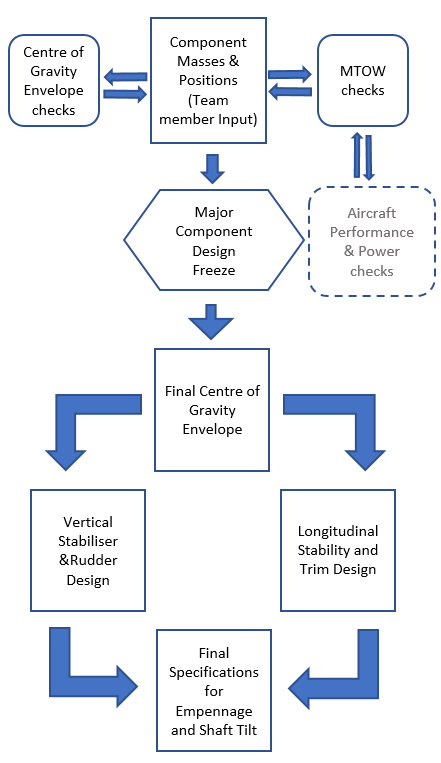
\includegraphics[width=8cm]{Flowchart.PNG}
\end{center}
    \caption{Overview of design process}
    \label{fig:flow}
  %  \vspace{-510pt}
\end{wrapfigure}
The remainder of this report is structured as follows. Section 2 provides the  context to the design specialisation of Weight, Balance, Stability \& Control with respect to the project as a whole. Section 3 presents the mass considerations including centre of gravity and moments of inertia. Section 3 provides the date needed for trim and empennage. Section 4 addresses passenger comfort and power consumption in deciding the main rotor shaft tilt and horizontal stabiliser parameters. Section 5 describes the addition of an active vertical stabiliser rudder to damp yaw oscillations. Section 6 discusses the design concluding with a reflection and a summary.
%-------------------------------------------------------------------------------
% TECHNICAL OVERVIEW
%-------------------------------------------------------------------------------
\section{Technical Overview}
A brief overview of the key design processes for this specialisation can be seen in  Figure \ref{fig:flow}.
% \begin{figure}[H]
% 	\flushright
% 	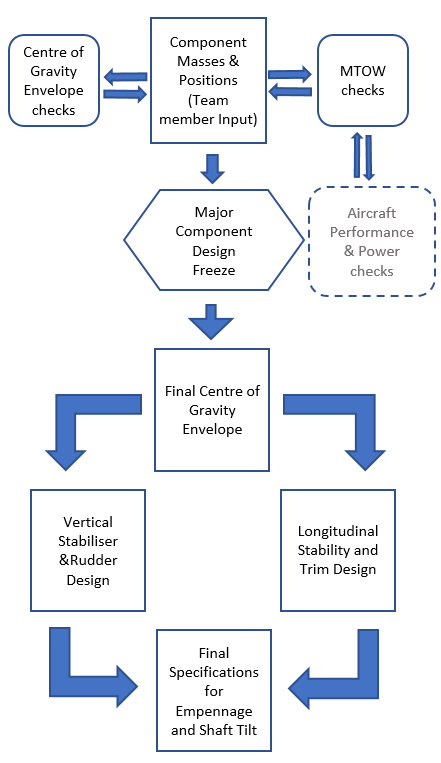
\includegraphics[width=0.4\textwidth]{Flowchart.PNG}
% 	\caption{Design process}
% 	\centering
% 	\label{fig:flowchart}
% \end{figure}


After the initial concept selection phase of the project, where it was decided what overall technologies and systems would be used, the focus was on completing a final design with technical justification that satisfied the requirements set by Leonardo and also internally. For this specialisation of weight \& balance, stability and control, this meant that tools had to be created to allow for trials and testing to be done to inform the design for every change in mass or mass location.

The information required from other specialisations are the masses and locations of said masses of the respective components. Initially broad estimates were used to gauge which components needed the most attention and as the project progressed more accurate estimates were provided. Every change to a component necessitated a re-evaluation of the mass properties of the aircraft which was then fed back into the specialisation providing them with the direction of whether the mass should be reduced or whether the location of such a part could be moved to improve the CG envelope. As the MTOW of the aircraft has such a large effect on the other specialisations the process of obtaining final masses was iterative. During this, the tools for creating the  CG envelope and trim conditions were developed using placeholder values for parameters which had yet to be determined.

It came to a point in the project where it was decided to freeze the specifications of the major components, namely the batteries, drive system, blades, cabin layout and structural members. So that final numbers could be calculated performance wise and to allow final design of trim and stability.
Once the design freeze had taken place, the masses and positions of each component were consolidated and that allowed the final CG envelope to be produced. This was done by obtaining the CG of the empty aircraft, and then permutating the layout of passengers and luggage to obtain the full range CG positions in 3D. This also allowed the minimum dimensions of the landing skids to be found. 

Next, longitudinal trim and shaft tilt had to be determined. This section constituted the most time consuming part of this specialisation. The shaft tilt and horizontal stabiliser design had to be determined simultaneously as both had to satisfy a sum of moments and forces. A parameter sweep of the shaft tilt and horizontal tail force was performed and the resulting longitudinal flapping angles and fuselage pitch were obtained for all CG positions found previously. A criteria was then formed to narrow down the selection to two configurations of shaft tilt and tail force, between these the optimum configuration was obtained. For the chosen design the resulting angles of fuselage and flapping for hover and cruise for a range of loading conditions were plotted. From the tail force it was possible to obtain a final design for the horizontal stabiliser.

Finally, the vertical stabiliser had to be designed. Unlike a penny-farthing the vertical stabiliser for a coaxial aircraft has to be modelled dynamically as it has no need to counter any resultant rotor torque statically in normal flight conditions. The stabiliser would be designed so as to meet a desired yaw damping ratio with considerations for size included. A dynamic model was created to simulate a static fin with which damping ratios could be obtained. A form of active rudder control was then implemented into the model to assess whether this option was desirable. A design was then decided upon that increased passenger comfort without an excessive increase in weight due to size.

%INSERT FANCY FLOWCHART
%\newpage
\section{Mass Distribution}
\subsection{Mass Breakdown}
% Describe how mass considerations influenced design process.
% Table of mass breakdown, pie chart
% Passenger and luggage loadout. configurations. CG affected in 3D. Show CG V loading. Show 3D plot.
% Say that median CG location used for trim design so that passenger comfort at extreme loadouts.
The mass considerations played a very important role in the design of this aircraft. The aim was to remain classified under CS-27 \cite{cs27} and the weight limit of SC-VTOL-01 \cite{scvtol}. This set a hard upper limit of 3175 kg. If this was exceeded then the aircraft would be classified under CS-29 which would entail a large redesign and possibly limit its usefulness in densely populated cities. In order to meet JAR-OPS3 requirement, the payload had to be set to 550 kg, which exceeds the project specified payload of 450 kg. \cite{jarops3}.


\begin{figure}[H]
\centering
		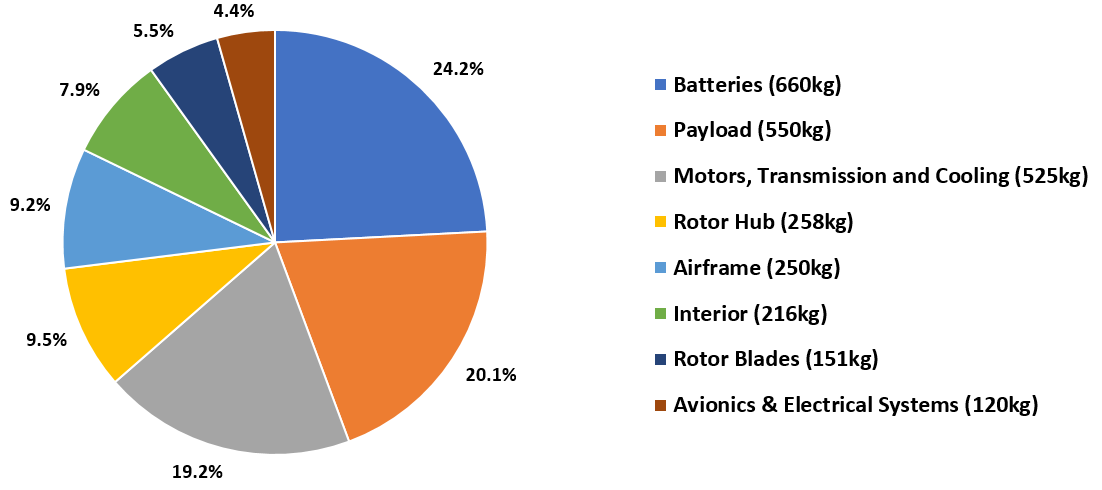
\includegraphics[width=0.8\textwidth]{PIE2.PNG}
		\captionof{figure}{Pie chart showing mass breakdown of components. A more detailed mass breakdown is in Appendix \ref{tab:massb}.}
		\label{fig:pie}
\end{figure}{}
% \begin{table}[H]
% 	\begin{minipage}{0.5\linewidth}
% 	\centering
% 		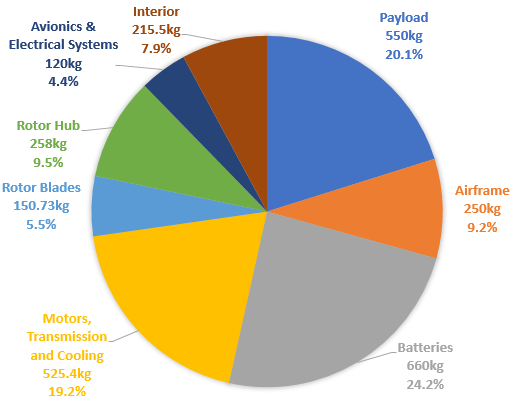
\includegraphics[width=\textwidth]{PIE.PNG}
% 		\captionof{figure}{Pie chart showing mass breakdown of components}
% 		\label{fig:pie}
% 	\end{minipage}\hfill
% 	\begin{minipage}{0.48\linewidth}
% 			\caption{Table of key weights}
% 		\label{tab:tabmass}
% 		\centering
% \begin{tabular}{lc}
%     \hline
%     \rowcolor[HTML]{DAE8FC} 
%     Weights       & kg   \\ \hline
%     Max Take-off Weight          & 2730 \\ \hline
%     Operational Weight Empty + Batteries & 2180 \\ \hline
%     Maximum Zero Fuel Weight         & 1070 \\ \hline
% \end{tabular}
% \begin{table}[H]
% \centering
% \caption{Table of Moments of Inertia}
% 		\label{tab:tabinertia}
% \begin{tabular}{cc}
% \hline
% \rowcolor[HTML]{DAE8FC} 
% Moments of Inertia & kgm$^2$   \\ \hline
% $I_{y_{CG}}$        & 3574.35 \\ \hline
% $I_{x_{CG}}$        & 2455.47 \\ \hline
% $I_{z_{CG}}$        & 1118.88 \\ \hline
% \end{tabular}
% \end{table}
% 	\end{minipage}
% \end{table}

The final mass breakdown and key weights can be seen in Figure \ref{fig:pie} and Table \ref{tab:tabmass} respectively. The largest mass by far are the batteries in this electrically powered aircraft.

\begin{table}[H]
	\begin{minipage}{0.5\linewidth}
	\caption{Key weights of aircraft}
		\label{tab:tabmass}
		\centering
\begin{tabular}{lc}
    \hline
    \rowcolor[HTML]{DAE8FC} 
    Weights       & kg   \\ \hline
    Max Take-off Weight          & 2730 \\ \hline
    Operational Weight Empty + Batteries & 2180 \\ \hline
    Maximum Zero Fuel Weight         & 1070 \\ \hline
\end{tabular}
	\end{minipage}\hfill
	\begin{minipage}{0.48\linewidth}
\centering
\caption{Moments of Inertia of unloaded aircraft}
		\label{tab:tabinertia}
\begin{tabular}{cc}
\hline
\rowcolor[HTML]{DAE8FC} 
Moments of Inertia & kgm$^2$   \\ \hline
$I_{y_{CG}}$        & 3574.35 \\ \hline
$I_{x_{CG}}$        & 2455.47 \\ \hline
$I_{z_{CG}}$        & 1118.88 \\ \hline
\end{tabular}

	\end{minipage}
\end{table}
\subsection{Moments of Inertia}

\begin{wrapfigure}[10]{r}{5.4cm}
\begin{center}
    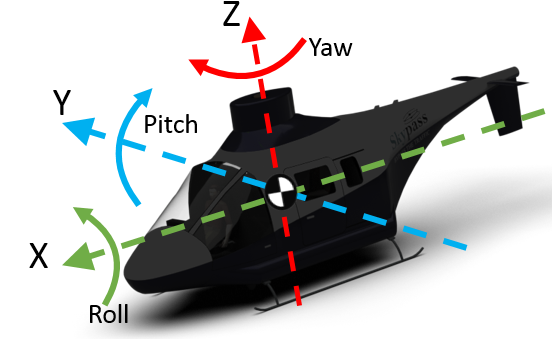
\includegraphics[width=5cm]{AXIS.PNG}
\end{center}
        \caption{Figure showing axis directions}
    \label{fig:axis}
  %  \vspace{-510pt}
\end{wrapfigure}
The calculation for the moments of inertia assumed point masses for each of the components, located at the best estimate of its centre of mass. The equation used to calculate the mass moment of inertia is in Appendix \ref{eq:izz}.

The moments of inertia around each of the 3-axis of the empty helicopter is in Table \ref{tab:tabinertia}. The largest moment of inertia is around the $y$-axis of motion, suggesting that the aircraft will resist pitching motion the most and then the rolling motion, with yawing being the easiest to enact.


\subsection{Centre of Gravity Envelope}
Following the finalisation of component masses and positions, the centre of gravity range, as it varies with payload loadout, was calculated in 3D. The assumptions were that each human being weighed 90 kg, and each passenger had the option of carrying up to 25 kg of luggage each. This formed the total payload mass of 550 kg. Every component was assumed to be a point mass. For every flight case the pilot was assumed present.
The longitudinal CG against AUW can be seen in Figure \ref{fig:CG1} and the 3D CG envelope can be seen in Figure \ref{fig:CG2}.

\begin{figure}[H]
\centering
\begin{minipage}{.5\textwidth}
  \centering
  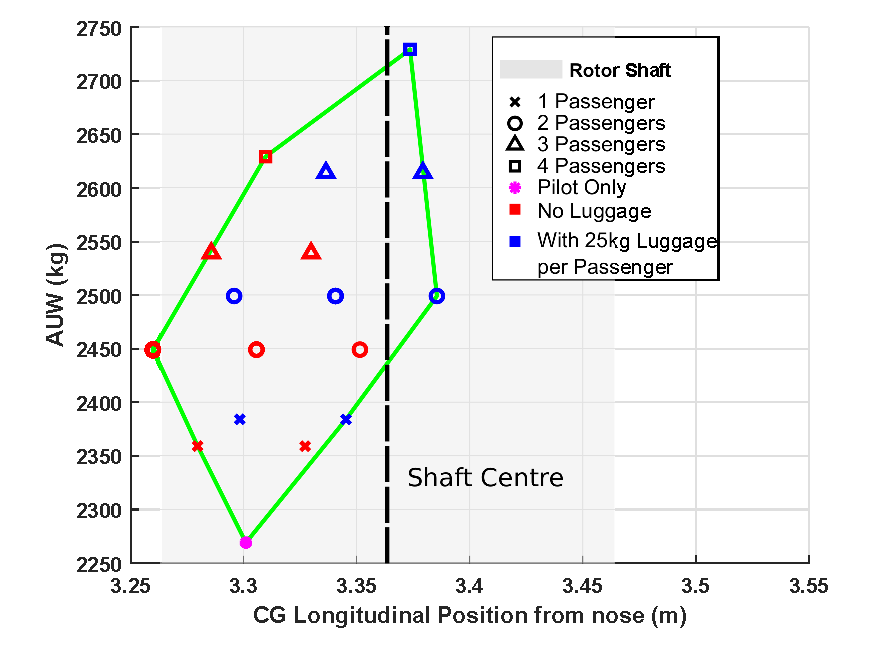
\includegraphics[width=\linewidth]{CGLONGVAUW.eps}
  \captionof{figure}{Longitudinal CG ($x$-axis) versus AUW.}
  \label{fig:CG1}
\end{minipage}%
\begin{minipage}{.5\textwidth}
  \centering
  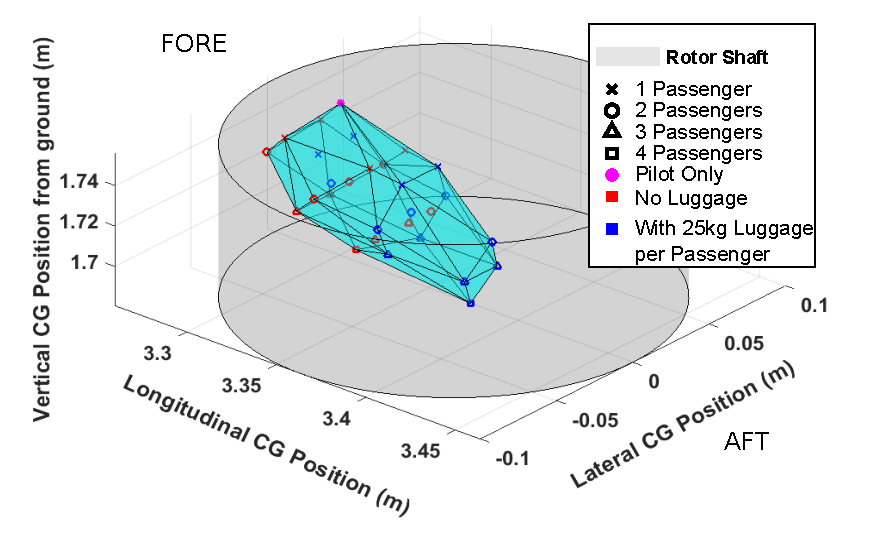
\includegraphics[width=\linewidth]{CG3D.eps}
  \captionof{figure}{3D CG Envelope}
  \label{fig:CG2}
\end{minipage}
\end{figure}

It was found that the CG location when empty lay 3mm forward of the centre of the main shaft and the largest deviation case consisted of 3 passengers, two in the front and one at the rear without any luggage, this is the leftmost point in Figure \ref{fig:CG1}. This resulted in a maximum deviation of 10.5cm forward of the main rotor, which is the preferred direction for stability and is relatively small\cite{prouty}. As can been seen in Figure \ref{fig:CG2}, in all except one case, the CG lies within the 20 cm diameter rotor shaft (shown as the cylindrical shaded region). From this, it is advisable that when loading the aircraft to direct passengers to fill the rear seats first. Lateral ($y$-axis) and vertical ($z$-axis) CG envelopes can be seen in Appendix \ref{fig:CGlat}.

This favourable CG envelope was a result of placing the heaviest components (See mass breakdown in Figure \ref{fig:pie}), such as the transmission, batteries and motors as close to the centre of the cabin as possible. During the design process it became evident that for structural reasons the main rotor would be better placed in the centre of the cabin. This was to ensure the structural member connecting the gearbox to the front of the cabin wasn't prone to buckling, for more details see structures specialisation report. To achieve this, the centre of mass had to be moved forward to be in line with the rotor shaft and so a trade study was drawn up to assess whether moving the heaviest component, the batteries, from it's original position of behind the cabin to below the cabin was the most viable solution. Table \ref{fig:batterypos} shows the outcome of this exercise where it was decided to position the batteries under the cabin floor. . The scoring was conducted through consensus, the higher the score the better that location was for that particular criteria. 

\begin{table}[H]
    \centering
    \caption{Trade study to decide position of battery}
    \begin{tabular}{c}
	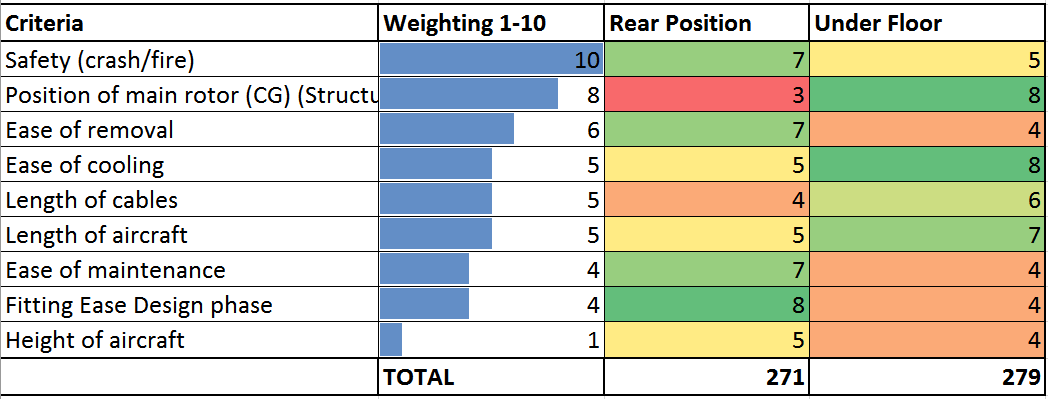
\includegraphics[width=0.8\textwidth]{batterypos.PNG}
    \end{tabular}
    \label{fig:batterypos}
\end{table}{}

\subsection{Ground Stability}
\begin{wrapfigure}[15]{r}{5.4cm}
\begin{center}
    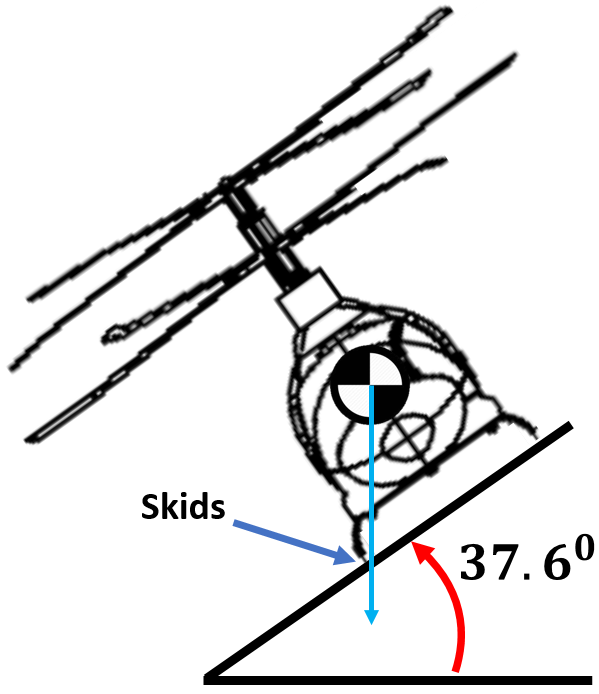
\includegraphics[width=5cm]{skids.PNG}
\end{center}
        \caption{Diagram showing maximum inclination of aircraft on ground}
    \label{fig:skids}
  %  \vspace{-510pt}
\end{wrapfigure}
The CG range information was used to inform the design of the helicopter skids so as to satisfy the 12 degree inclination requirement. 
The skids require input from three specialisations, weight and balance, structures and rotor design. The skids had to have dimensions such that the CG is within their footprint even at a 12 degree incline on the ground, this provided the minimum dimensions required. This was then passed on to the structures and rotor specialisms to ensure that they could support the aircraft and ensure that the frequency of the rotors did not resonate with the aircraft on the ground.

Following this, the final skids allow for an on-ground inclination of 37.6 degrees where the CG lies just within the skids. This is assuming worst case CG scenario of no payload, where the CG is highest from the ground. Figure \ref{fig:skids} shows the maximum inclination possible with final design of the skids, the orientation shown is the limiting direction. \\
%-------------------------------------------
% CHAPTER: SHAFT TILT AND HORIZONTAL STABILISER
%-------------------------------------------
\section{Shaft Tilt and Horizontal Stabiliser}
\subsection{Overview}
The aim of this section is to maximise passenger comfort and reduce power consumption through trim and empennage specifications. Increasing passenger comfort can be done by minimising the fuselage pitch deviation from zero in both hover and cruise. Reducing power consumption can be done by minimising the flapping angles.
\begin{figure}[H]
    \centering
    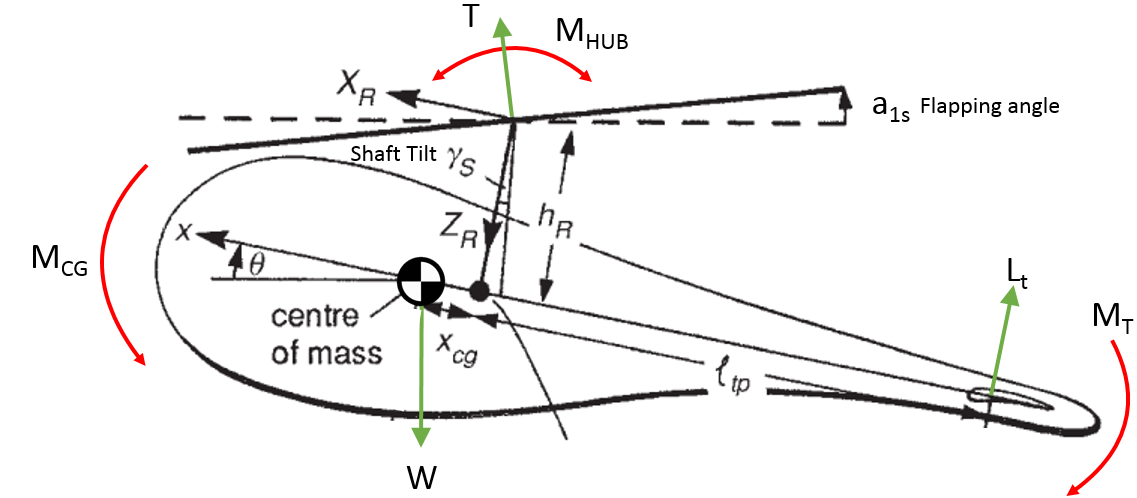
\includegraphics[width=0.8\textwidth]{FBD.PNG}
    \caption{Side view schematic showing key forces and moments (adapted from Padfield \cite{padfield})}
    \label{fig:fbd}
\end{figure}{}

During forward flight the rotor must tilt forward to balance the forces generated by the drag of the fuselage.
In a typical helicopter with zero shaft tilt and an articulated hub the fuselage would also tilt forward slightly with the rotor disc, with the remainder of the tilt being fulfilled by the rotor flapping angle. 
However, large fuselage pitch angles are not very comfortable and so it is possible to have the rotor shaft fixed at a forward angle reduce fuselage pitch during cruise. This does have the drawback of increasing the fuselage pitch and flapping angle during hover and so a balance must be struck.

In addition, rotors with a blade hinge offset are able to impart moments onto the aircraft, this hub moment is proportional to the flapping angle and this derivative can be described by Equation \ref{eq:hubmom}:
\begin{equation}
    \frac{dM_m}{da_{1s}}=0.25*(e/R)*b\,m_b\,R*(\Omega\,R^2) \label{eq:hubmom}
\end{equation}{}
where $e$ is the blade hinge offset ratio\cite{prouty}.
This is beneficial as it allows the aircraft to counter the moment created by not having a centre of mass exactly below the line of action of the rotor. This means it is able to force the fuselage to stay relatively parallel to the ground even in unfavourable CG conditions, much more so than if there was no hinge offset in which case the aircraft would simply tilt until the CG was directly under the main rotor. In this project, the hinge offset was calculated by the rotor blade and rotor hub specialists so as to reduce resonance and vibration. Details of its determination can be found in those reports.

This effect is mainly helpful during hover, where the only constraint is that the tip path plane of the rotor must remain parallel to the ground allowing the flapping angle to be adjusted to balance the moment from the CG offset, of course the resulting fuselage pitch is highly dependant on shaft tilt. In cruise, the tip path plane has the additional constraint of balancing of forward thrust and drag, meaning that the tip path plane is now angled forward. Now the resulting hub moment may only allow the fuselage to be 'corrected' to a certain degree, again dependant on shaft tilt, meaning that the pitch angle may not be ideal. This is where the addition of a horizontal stabiliser is helpful. A horizontal stabiliser during cruise is able to generate a moment which can work in tandem with the moment of the rotor flapping angle to reduce fuselage pitch.

To summarise, the two aircraft specifications that need determining are the rotor shaft tilt ($\gamma$) and the moment generated by the horizontal stabiliser ($M_t$). The effect of these on the resulting fuselage pitch angles ($\theta_f$) in both hover and cruise, and the required flapping angles ($a_{1s}$) also in both hover and cruise need to be analysed and then a method of optimisation needs to be employed to obtain the best compromise of $\gamma$ and $M_t$.

Another layer of complexity arises when it becomes necessary to account for the varying location of CG for different payload configurations. Ensuring that the resulting characteristics of the aircraft are acceptable for all possible payload combinations is important as it must be able to remain viable in the varying situations it is likely to encounter being a public transport vessel.
\subsection{Assumptions}
\subsubsection{Longitudinal}
The equations used for longitudinal stability and trim are adapted from Prouty \cite{prouty}, these equations are built on several assumptions:

\begin{itemize}
    \item Reverse flow region neglected.
    \item Tip loss and root cut out neglected.
    \item Small angles are assumed.
\end{itemize}{}

To simplify calculations further, additional assumptions have been made:

\begin{itemize}
    \item The rotor thrust vector is perpendicular to the tip path plane
    \item The two main 4-bladed rotors are assumed to flap in the same direction with equal magnitude therefore acts as a single rotor for trim purposes.
    \item Rotor downwash effects on drag of fuselage and empennage are ignored in calculations.
    \item Fuselage pitching moment and lift ignored.
    \item Minimum drag condition of fuselage assumed zero pitch.
\end{itemize}{}

In the absence of full CFD and/or wind tunnel testing, the aerodynamic characteristics of the fuselage have been ignored with the exception of flat plate drag, $D_{f_X}=1.84V^2$, this was obtained using conditions at cruise altitude.
The location of the horizontal stabiliser has been placed $5$ meters behind the centre of the cabin so that the downwash from the rotors would have a reduced affect. This means that the variable $M_t$ can be reduced to $L_t$ as $M_t=L_t\cdot l_t$. The coning angle of the rotors has been ignored as they do not produce a resultant moment that would affect trim.

The equations used can be seen in Appendix \ref{eq:trimeq}\\


\subsubsection{Lateral Consideration}
A note on lateral stability and trim, unlike a penny-farthing a coaxial helicopter does not suffer from the lateral stability issues caused by the presence of a tail rotor, i.e side-slip, gust alleviation issues etc. Therefore, the lateral stability considerations are almost identical to that of longitudinal with the exception of that fact that the requirements in this direction are much reduced, CG positions change very little laterally and rotor flapping has no additional constraints either as the aircraft is not expected to fly sideways at any significant speed.
It can be said then that if the aircraft performs acceptably longitudinally then lateral stability should not be an issue as lateral flapping angles (flapping would be the aircraft's only way to exert lateral control) would be much less than longitudinal.

\subsection{Data Generation}
To be able to explore the relationships between the two input variables ($\gamma,L_t$) and the  four output variables ($a_{1s_{hover}},a_{1s_{cruise}},\theta_{f_{hover}},\theta_{f_{cruise}}$) for each CG position, a parameter sweep was performed.

The range of input values was a Shaft Tilt, $\gamma$, from $0$ to $-9$ degrees and a Tail lift, $L_t$ of $0$ to $900N$. This range was found to encompass the values of interest, i.e results that span across the zero angle planes, and also values that typical helicopters employ \cite{prouty}.

Initially the median CG position was used to obtain initial values, which were the results presented at FDR, and to allow sanity checks to be made. However, for any particular configuration of shaft tilt and tail force, the fuselage pitch angles and rotor flapping angles will change depending on the location of CG. Therefore, in order to obtain the maximum and minimum values that could be experienced by the aircraft each configuration had its full range of CG positions evaluated for with the maximum and minimum values for each configuration stored.

\subsection{Results}

The maximum and minimum values for pitch angles and flapping angles for both cruise and hover as CG is varied across its range were plotted against shaft angle and tail force. Two surface plots for cruise and two 2D plots for hover, as tail force has no effect on the hover condition, were produced. These can be seen below:

\begin{figure}[H]
\centering
\begin{minipage}{.48\textwidth}
  \centering
  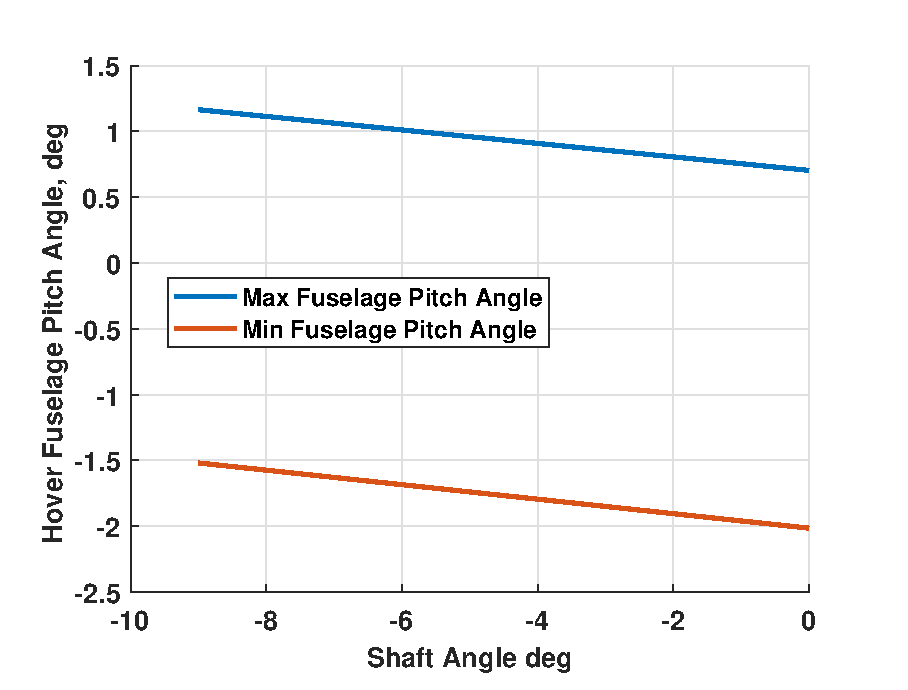
\includegraphics[width=\linewidth]{hovershaftpitch.eps}
  \captionof{figure}{Figure showing how fuselage pitch angles change with shaft tilt in hover}
  \label{fig:hshaftpitch}
\end{minipage}\hspace{0.2cm}
\begin{minipage}{.48\textwidth}
  \centering
  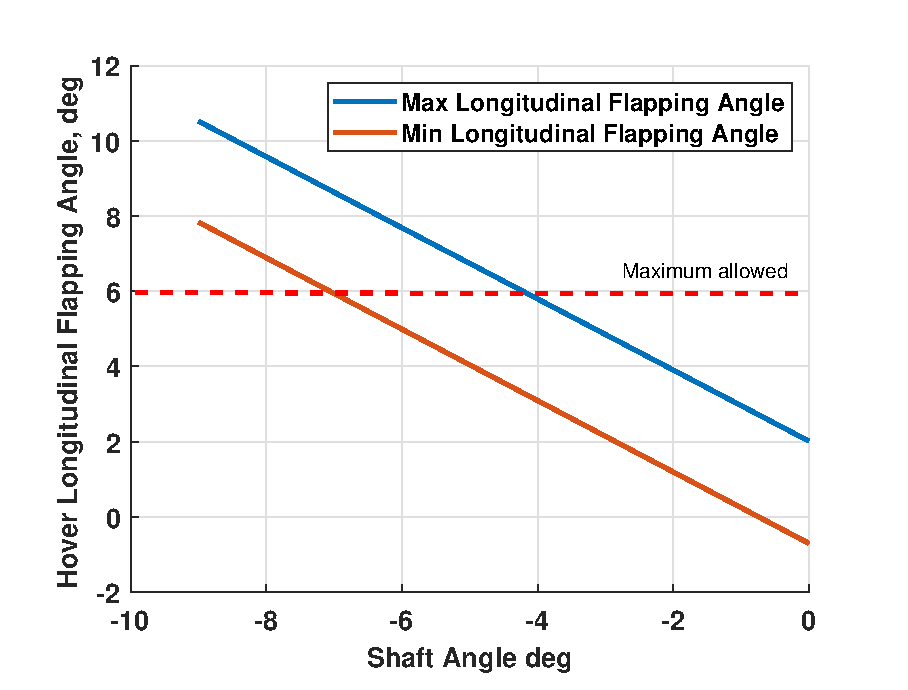
\includegraphics[width=\linewidth]{hovershaftflap.eps}
  \captionof{figure}{Figure showing how longitudinal flapping angles change with shaft tilt in hover}
  \label{fig:hshaftflap}
\end{minipage}
\end{figure}
\begin{figure}[H]
\centering
\begin{minipage}{.49\textwidth}
  \centering
  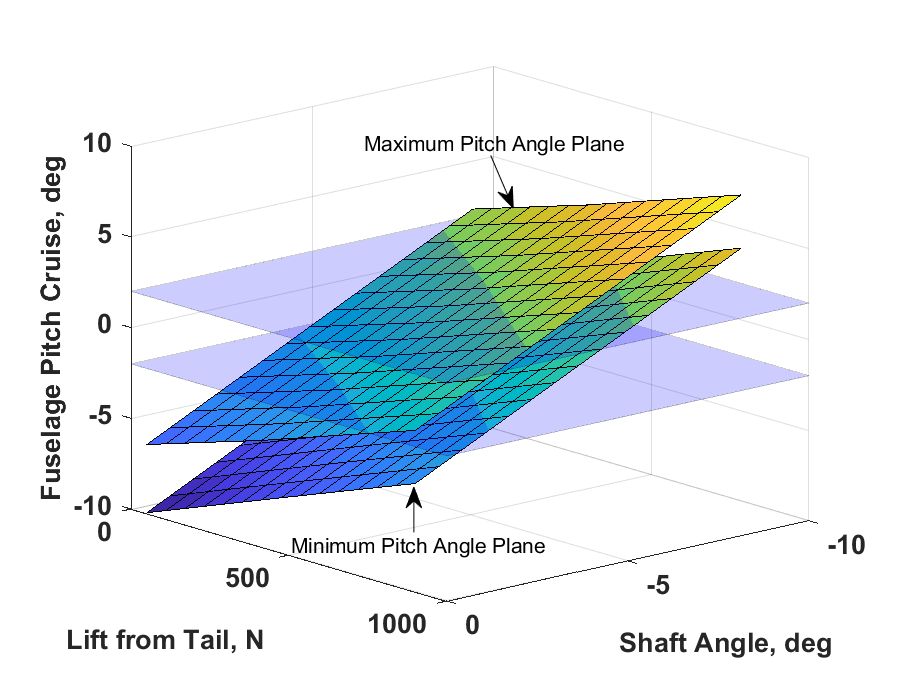
\includegraphics[width=\linewidth]{cruisepitch.eps}
  \captionof{figure}{Figure showing how cruise fuselage pitch angles change with shaft tilt  and tail force in cruise}
  \label{fig:cruisepitch}
\end{minipage}\hspace{0.2cm}
\begin{minipage}{.49\textwidth}
  \centering
  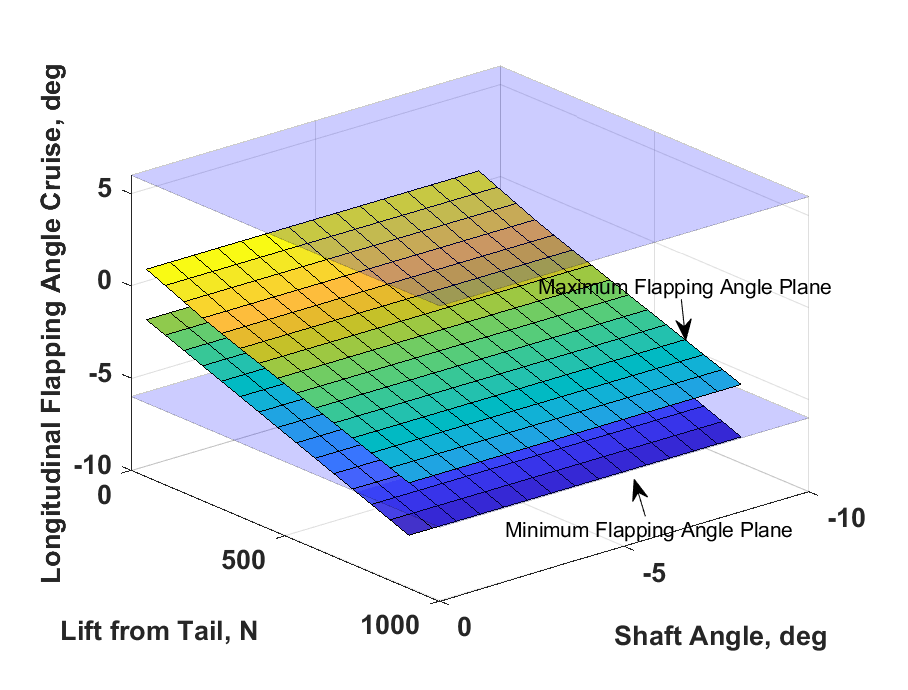
\includegraphics[width=\linewidth]{cruiseflapping.eps}
  \captionof{figure}{Figure showing how longitudinal flapping angles change with shaft tilt and tail force in cruise}
  \label{fig:cruiseflap}
\end{minipage}
\end{figure}
It is clear from the above figures that the individual relationships are approximately linear.
From Figure \ref{fig:hshaftpitch}, it can be seen that increasing the forward tilt of the rotor shaft results in increasing the nose-up pitch during hover. Figure \ref{fig:hshaftflap}, shows a similar trend with the hover flapping angle, this flapping angle proved to be the limiting factor when increasing shaft tilt.

From Figure \ref{fig:cruisepitch} it can be seen the both shaft tilt and tail force have the same effect of linearly increasing the pitch angle of the fuselage in cruise. In Figure \ref{fig:cruiseflap}, it can be seen that the shaft angle has minimal effect on the flapping angle, this is expected as during cruise the shaft tilt only serves to bring up the nose. It also shows that as $L_t$ increases the longitudinal flapping angles decreases. This trend limited the maximum $L_t$ allowed.

It is not straightforward to state that increasing a particular parameter is desirable for a certain result as it depends on the starting point from which you choose to vary.


\subsection{Configuration Selection}


Following this data gathering, the challenge was to create a method to find the best solution, or a solution that best satisfied a criteria. Many methods of optimisation were attempted that tried to minimise fuselage pitch angles while also minimising flapping angles. The method presented here is to rule out combinations of $\gamma$ and $L_t$ that resulted in values that exceeded a threshold.

To do this a criteria was formed:

\begin{itemize}
    \item A fuselage pitch angle of up to $\pm2$ degrees would be allowed in all conditions this is judged to be imperceptible to the passenger.
    \item Maximum flapping angle allowed in all conditions is $\pm6$ degrees, this is considered a large flapping angle \cite{prouty}\cite{padfield}.
\end{itemize}{}

These limitations are visualised in the above figures through boundary planes in the surface plots and dashed lines in Figure \ref{fig:hshaftflap}.
This resulted in only two out of the $225$ tested combinations satisfying the constraint:

\begin{table}[H]
\centering 
    \caption{Table showing final cases that satisfy criteria}
\begin{tabular}{ccc}
\hline
  \rowcolor[HTML]{DAE8FC} 
  Parameter & Case 1 & Case 2\\ \hline
   Shaft Tilt, $\gamma$ & $-3.86$ deg & $-3.86$ deg\\
   Tail Force, $L_t$ & $657.14N$ & $717.86N$\\
   \hline
\end{tabular}{}
    \label{tab:long}
\end{table}{}

The only differing value between the cases in Table \ref{tab:long} is the Tail Force, suggesting differing cruise characteristics. The cruise characteristics of the two cases were plotted together, Figure \ref{fig:cases}, and as the relationship between the individual parameters has been observed to be linear the points were joined by a straight line.
\begin{figure}[H]
    \centering
    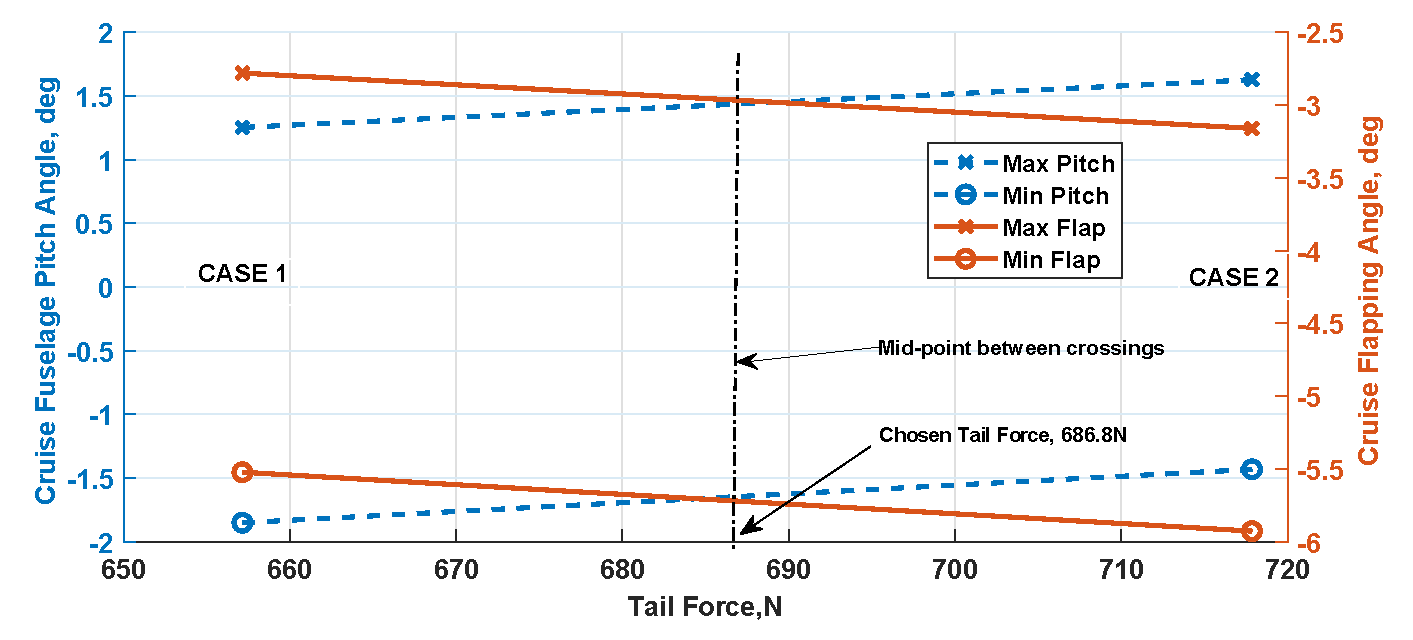
\includegraphics[width=0.9\textwidth]{cases.eps}
    \caption{Figure showing combined cruise results of both qualifying cases v. Tail Force and the final value of tail force selection method}
    \label{fig:cases}
\end{figure}{}
This plot allowed the crossings of the maximum angles and minimum angles to be found. Ordinarily a double plot could not be used to directly relate two variables to each other, however, as the $y$-limits have been approximately matched graphically the crossings observed would correspond roughly to a minimum of the two. The Tail force chosen was the mid point of these crossings which can be seen in Figure \ref{fig:cases}. This can be said to be the optimum Tail force for this shaft tilt, assuming the flapping and pitch angles are weighted equally at this stage. Thus, the final configuration is a Shaft Tilt of $\gamma=-3.86$ degrees and a Tail Force of $L_t=686.8N$.

The resulting maximum and minimum pitch angles and flapping angles can be seen in Table \ref{tab:cgres}, while full results for each CG location can be seen in plots in Appendix \ref{fig:CGHOVERP}.
\begin{table}[H]
\centering
\caption{Table showing limits of rotor flapping and fuselage pitch angles for chosen design accounting for all CG positions}
\begin{tabular}{c|c|c|c|c|}
\cline{2-5}
                                                & \multicolumn{2}{c}{\cellcolor[HTML]{DAE8FC}Cruise}                             & \multicolumn{2}{c|}{\cellcolor[HTML]{DAE8FC}Hover}        \\ \cline{2-5} 
                                                & \multicolumn{1}{c|}{\cellcolor[HTML]{DAE8FC}Min} & \cellcolor[HTML]{DAE8FC}Max & \cellcolor[HTML]{DAE8FC}Min & \cellcolor[HTML]{DAE8FC}Max \\ \hline
\multicolumn{1}{|l|}{Fuselage Pitch Angle, deg} & \multicolumn{1}{c|}{-1.65}                       & 1.44                        & -1.80                       & 0.90                        \\ \hline
\multicolumn{1}{|l|}{Long. Flapping Angle, deg} & \multicolumn{1}{c|}{-5.72}                       & -2.96                       & 2.96                        & 5.66                        \\ \hline
\end{tabular}
\label{tab:cgres}
\end{table}
From this value of tail force it was possible to obtain the specifications of the horizontal stabiliser. The equation for lift is $L_t=\frac{1}{2}\rho V^2 S_h C_{l_\alpha}(\theta_f+\phi_{setting})$, NACA2410 was chosen based on it's high lift/drag ratio and high $C_{l_\alpha}$. The previous code also included the drag of the stabiliser as the setting angle is varied,for a set $S_h$. This area was decided based on observing existing helicopters' size proportionally to the main rotors. The code produced a setting angle that would be required to fulfil trim. The final specifications can be seen in Table \ref{tab:longfinal}.

\begin{table}[H]
\centering 
    \caption{Table showing final specifications}
\begin{tabular}{lc}
\hline
  \rowcolor[HTML]{DAE8FC} 
  Parameter & Value \\ \hline
   Shaft Tilt, $\gamma$ & $-3.86$ deg\\
   Tail Force, $L_t$ & $686.8N$\\
   Aerofoil of H. Stabiliser & NACA2410\\
   Area of H. Stabiliser & $0.61m^2$\\
   Setting Angle, $\phi_h$ & $-9.8$ deg\\
   \hline
\end{tabular}{}
    \label{tab:longfinal}
\end{table}{}

% It was decided to optimise for minimising the delta between fuselage tilt in hover and in cruise. This allows the option the tilting seating to compensate for a near constant fuselage tilt throughout the journey. The absolute values will be checked after to ensure on ground tilt is not extreme. A surface plot of this delta, $\theta_{f_{hover}}-\theta_{f_{cruise}}$, can be seen in Figure ADDREF.

% Two points were selected along the intersection of this surface and the zero plane and were used to derive the equation of the line that represents the configurations optimised for pitch delta, $\gamma=h(L_t)$.

% Next, for each of these configurations the energy consumption due to flapping actuation were calculated and a minimum found.
% The cost function for energy is as follows:
% \begin{align}
%     \text{Energy Consumption}&=f(a_{1s_{cruise}},a_{1s_{hover}})\\
%     a_{1s_{cruise}}&=g(\gamma,L_t)\\
%     a_{1s_{hover}}&=g_h(\gamma)
% \end{align}{}
% However, as $\gamma$ and $L_t$ are now dependant variables the substitution of $\gamma=h(L_t)$ can be made leading to:
% \begin{align}
%     \text{Energy Consumption}&=f(g(h(L_t)))
% \end{align}{}
% The functions $g$ and $h$ are known but assumptions have to made to obtain a relationship for $f$. It is assumed from the mission profile that only $10\%$ of the average journey would be in hover while the other $90\%$ would be in cruise. And that as flapping actuation increases energy consumption increases linearly. Therefore, it could be said that for a typical journey:

% \begin{align}
%         \text{Energy Consumption}&\propto 0.9*a_{1s_{cruise}}+0.1*a_{1s_{hover}}
% \end{align}{}

\subsection{Discussion}
The aim was to ensure passengers remain comfortable during flight and that the power used to maintain that comfort was not excessive. 
The objectives to achieve this aim was to determine a shaft tilt and a horizontal stabiliser design that served to minimise the fuselage tilt during cruise while not sacrificing that in hover and to ensure the flapping angles required to maintain trim were not large. This presented a challenge in optimisation. The method presented here was to narrow down cases until those that satisfied a criteria was found, then find the middle ground of those cases. Many alternative methods of optimisation were attempted although yielded results that were not satisfactory, due to time constraints these methods could not be explored further. What was attempted was the use of a cost function that directly related energy use and passenger comfort to the shaft angle and tail force. However, with the lack of information of the relationship between energy consumption and flapping angles as well as tweaking the function to weigh cruise and hover conditions differently, this proved time consuming. 

The results presented here differ slightly from what was presented at FDR, this is due to the addition of considering the full CG variation throughout the entire analysis rather than a verification at the end. Otherwise, the process followed is largely the same. 

The results of the chosen design succeed in meeting the criteria set. The maximum fuselage pitch deviation possible is $-1.80$ degrees during hover, from Appendix \ref{fig:CGHOVERP} it can be seen that this represents the aircraft when only the pilot is present. As SkyPass 3 is predicted to be operating using a point-to-point model, where the landing sites are pre-determined and are large transport hubs, this situation of flying with the pilot only is not expected to be the norm, unlike an existing taxi service where the vehicle would have to make return journeys or travel to passenger pick-up points empty. In the case of SkyPass 3, the aircraft will await the arrival of a passenger wherever it is landed, minimising flying empty.

The rotor flapping angles have a maximum angle of $-5.72$ degrees which is below the $6$ degree threshold set internally, however, this is assumed for single rotor. Skypass 3 is a coaxial helicopter and therefore this angle can be halved for both rotors, possibly allowing even larger total flapping angles to be used, however, as to whether deflecting two rotors by a small angle is more power efficient than deflecting a single rotor by a large angle is not clear.

Future work would focus on improving the applicability of the model to a coaxial configuration, as well as investigating the relationship between flapping angles and energy consumption. Future work would also be done on improving the methods of selecting the final configuration of shaft tilt and horizontal stabiliser. A suggestion would be to extract the linear relationships between each parameter and result and obtain an optimum through linear programming.





\section{Vertical Stabiliser Sizing}

% Describe purpose of Vstab in coaxial. 
% Dynamic analysis required.
% Show equations, assumptions
% Show how actuation was added.

% Show resulting plots, sizing.
\begin{wrapfigure}[15]{r}{5.5cm}
    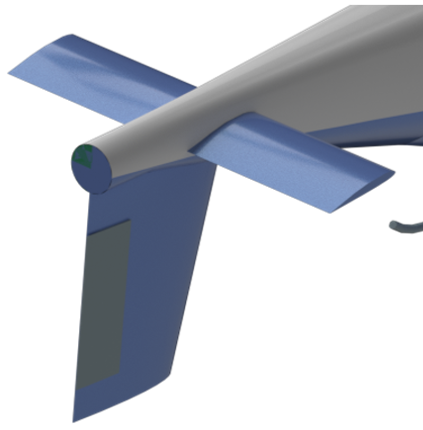
\includegraphics[width=5cm]{Empennage.png}
    \caption{SkyPass 3 Empennage }
    \label{fig:emp}
    %\vspace{-510pt}
\end{wrapfigure}
In a conventional penny-farthing helicopter the vertical stabiliser may be designed to offload the tail rotor during forward flight. However, in a coaxial helicopter where the counter-rotating rotors produce no resultant torque the vertical stabiliser plays no role in static stability. Instead, it's main purpose would be to damp out yaw disturbances through the "weather-vane" effect, increasing passenger comfort. Therefore, it was necessary to analyse the vertical stabiliser dynamically.


The design process was to create a dynamic model of the damping effects of the vertical stabiliser, use the model to obtain initial sizing for a desired damping ratio identified from literature, which is approximately 0.45 \cite{prouty}. Basic active rudder control was added to the model for comparison, allowing a decision to be made whether to opt for the actively controlled system or not for a specific damping ratio.
\subsection{Modelling}
\subsubsection{Vertical Stabiliser}
The dynamic model was created using the lift curve slope of NACA0006. The model excludes any effects of the main rotors and damping effect of the fuselage, small angles are assumed. The yaw moment of inertia of the helicopter,$I_{zz}=1118.8 kgm^2$ was used. The quarter-chord of the fin was placed $5m$ behind the CG of the helicopter ($l=5$m) to avoid downwash effects. 
\begin{figure}[H]
	\centering
	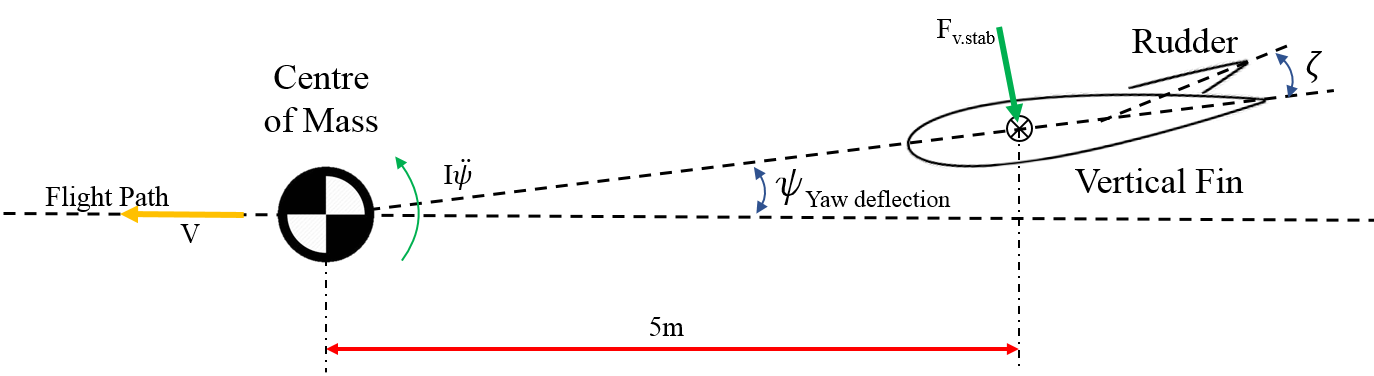
\includegraphics[width=0.9\textwidth]{VertStabdiag.PNG}
	\caption{Plan view of dynamic model of vertical stabiliser}
	\centering
	\label{fig:vertdiag}
\end{figure}

Based on the diagram in Figure \ref{fig:vertdiag}, excluding the rudder, the equation of motion was derived:
%\begin{align}
%\Sigma M: I_{ZZ}\ddot{\psi}&=l(\frac{1}{2}\rho V^2 %S_{tp}C_L(\psi+\frac{\dot{\psi}l}{V})) \\
%\text{let,}\,\, A&=\frac{1}{2}\rho V^2 S_{tp}C_L\\
% \text{therefore,}\,\,I_{ZZ}\ddot{\psi}&=\frac{Al^2}{V}\dot{\psi}+A l\psi %\label{eq:eom1}
%\end{align}{}
\begin{equation}
    \Sigma M: I_{zz}\ddot{\psi}=l(\frac{1}{2}\rho V^2 S_{tp}C_L(\psi+\frac{\dot{\psi}l}{V})), 
\end{equation}
let
$A&=\frac{1}{2}\rho V^2 S_{tp}C_L$,
therefore
\begin{equation}
   I_{zz}\ddot{\psi}=\frac{Al^2}{V}\dot{\psi}+A l\psi \label{eq:eom1} 
\end{equation}


\subsubsection{Active Rudder Control}

To observe the effects a form of active rudder control could have on the system, the following additional assumptions were made:

\begin{itemize}
\item The deflection of the rudder is equal to the deflection of the aircraft (i.e., $\psi=\zeta$). This is only true for small angles. 
\item The rudder occupies a third of the area of the vertical stabiliser, which was assessed to be sufficient to house the mechanism and limits the power consumption by not using the entire area. 

\item The control time delay is assumed instant. This is unrealistic but for the purposes of this project and considering the time constraints this was deemed to be a satisfactory simplification. 

\item The difference in the location of the force generated by the rudder and by the vertical fin is assumed zero. This was assessed to be a relatively valid assumption as the difference would be small relative to $l$ and in any case would generate a more conservative result. Both use the same aerofoil, ($C_{L_{tp}}=C_{L_{r}}=C_L$).
\end{itemize}

This allowed a second equation of motion to be derived, again based on Figure \ref{fig:vertdiag}:
%\begin{align}{}
%\Sigma M: I_{ZZ}\ddot{\psi}&=l(\frac{1}{2}\rho V^2 S_{tp}C_L(\psi+\frac{\dot{\psi}l}{V})+\frac{1}{2}\rho V^2 S_R C_L(\psi+\frac{\dot{\psi}l}{V}+\zeta+\frac{\dot{\zeta}l}{V})) \\
%\text{let,}\,\,A&=\frac{1}{2}\rho V^2 C_L\,;\, \psi=\zeta\\
% \text{therefore,}\,\,I_{ZZ}\ddot{\psi}&=A\,l\,\left(2\,S_{R}+\,S_{\mathrm{tp}} %\right) \psi+\frac{3\,A\,l^2\,S_{\mathrm{tp}}\,}{V} \dot{\psi} \label{eq:eom2}
%\end{align}{}

\begin{equation}
    \Sigma M: I_{zz}\ddot{\psi}=l(\frac{1}{2}\rho V^2 S_{tp}C_L(\psi+\frac{\dot{\psi}l}{V})+\frac{1}{2}\rho V^2 S_R C_L(\psi+\frac{\dot{\psi}l}{V}+\zeta+\frac{\dot{\zeta}l}{V}))
\end{equation}
let $A&=\frac{1}{2}\rho V^2 C_L$ and $\psi=\zeta$, therefore
\begin{equation}
    I_{zz}\ddot{\psi}=A\,l\,\left(2\,S_{R}+\,S_{\mathrm{tp}} \right) \psi+\frac{3\,A\,l^2\,S_{\mathrm{tp}}\,}{V} \dot{\psi} \label{eq:eom2}
\end{equation}
\subsection{Results \& Discussion}
Equations \ref{eq:eom1} and \ref{eq:eom2} were simulated in Matlab and the damping ratios for each were obtained for a range of surface areas. This can be seen in Figure \ref{fig:vstab1}.

\begin{figure}[H]
\centering
\begin{minipage}{.48\textwidth}
  \centering
  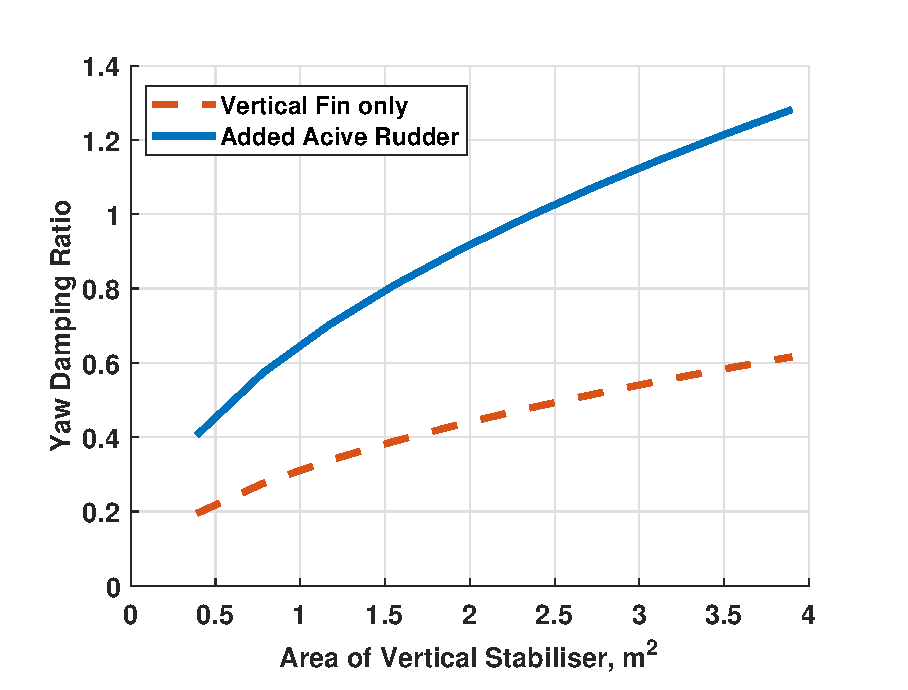
\includegraphics[width=\linewidth]{DampVArea3.eps}
  \captionof{figure}{Comparison of Yaw Damping Ratio between an active rudder and static fin.}
  \label{fig:vstab1}
\end{minipage}\hspace{0.2cm}
\begin{minipage}{.48\textwidth}
  \centering
  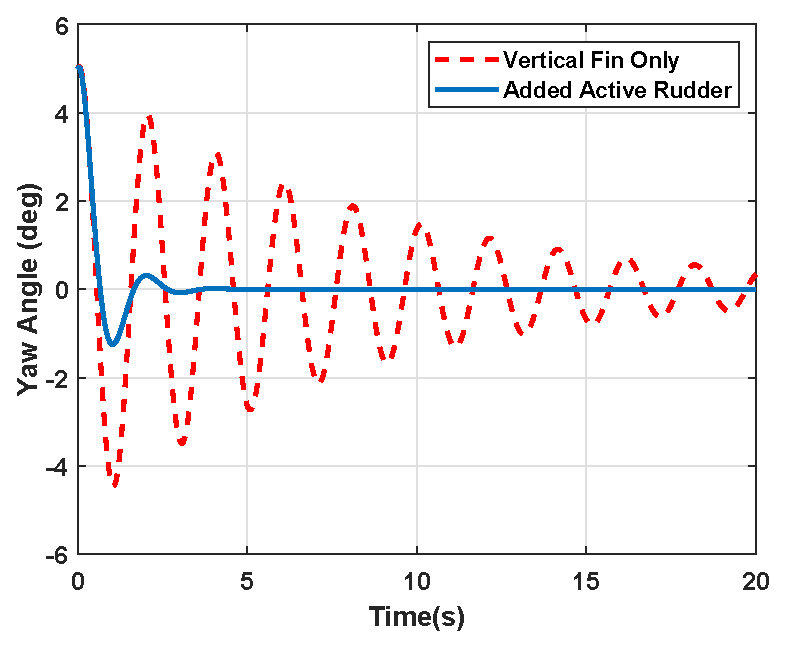
\includegraphics[width=0.9\linewidth]{Vstabresp2.eps}
  \captionof{figure}{Comparison of Time Response of active rudder with static fin}
  \label{fig:vstab2}
\end{minipage}
\end{figure}
 As can be seen from Figure \ref{fig:vstab1} the active rudder offers a much greater degree of damping for the same area. The damping was increased by 2.08 times in every case. To obtain the level of damping required, an area of 0.39 m$^2$ was chosen with rudder control. The time response comparison to that of no rudder and the same area can be seen in Figure \ref{fig:vstab2}.

The decision was made to have the vertical stabiliser mounted below the tail, this was to ensure that any lateral force generated by the fin would not induce a large rolling moment as the centre of pressure would be much more in line with the vertical location of CG, this can be seen in the GA. This does mean that the stabiliser could be less effective as it may be in the wake of the fuselage, however, this is less of an issue as it is not expected to be used during normal flying conditions as the aircraft employs differential torque of the rotors as its main method of yaw control. Any disturbance in yaw would increase the exposure of the stabiliser to the air and assist in damping. Another, is the case of auto-rotation, where the velocity vector is downwards meaning the stabiliser will not be blocked by the fuselage and will help in keeping the aircraft facing forward.

In all other cases, the vertical stabiliser is not considered a 'mission critical' surface, meaning it is not absolutely required to maintain normal flight in the case of a coaxial helicopter. It is implemented here to increase passenger comfort and handling.
\begin{table}[H]
\centering 
    \caption{Parameters of Vertical Stabiliser}
\begin{tabular}{ll}
\hline
  \rowcolor[HTML]{DAE8FC} 
  Parameter & Value  \\ \hline
   Area  & 0.39 m$^2$\\
   Aerofoil & NACA0006\\
   Damping Ratio & 0.404\\
   Position from Cabin centre & 5 m\\
   \hline
\end{tabular}{}
    \label{tab:vstab}
\end{table}{}
Future work may be done to assess the rudder's use as a method of yaw control that may or may not have a energy saving effect by  reducing the role of the main rotors in this. Further, the considerations and assumptions of the models may be improved to allow more accurate data to be produced to better inform the design. Namely, a more realistic control system, effects of the fuselage and rotors during a yaw deflection could be implemented as well as model verification through wind tunnel testing.
%
% Summary and Conclusions
%

% Reflection
% --------------------
\section{Summary}
location of masses, position and tilt of main rotor, active rudder. Is this basically the outputs of the design?

The relevant mass considerations were taken into account to 



\section{Reflection}

Teamwork

Engineering challenge, compromise.

large number of assumptions

communication
 regular meetings


*** WHAT WOULD YOU DO DIFFERENTLY? INTERACTIONS WITH GROUP/SUPERVISOR.***
*** WHAT WENT WELL ***
*** WHAT DIDNT GO WELL AND WHAT COULD HAVE BEEN DONE TO PREVENT IT IF PROJECT DONE AGAIN***
 The challenges of minimising weight through battery technology selection, motor selection, drive-train design, rotor design, etc proved to be a lengthy iterative process that benefited from creating tools that could be used to quickly check various aspects of weight and balance. 
Weights required input from team members, tests required close cooperation with performance specialist and battery and drive-train specialist. Feedback to rest of team.

Every major decision was done as a group with the help of trade study tables. Constant clear communication was key.


%-------------------------------------------------------------------------------
% REFERENCES
%-------------------------------------------------------------------------------
\begin{thebibliography}{}
\bibitem{prouty}R. Prouty, Helicopter performance, stability, and control. Malabar: Krieger Pub., 2005.
\bibitem{padfield} Padfield, Gareth D., et al. Helicopter Flight Dynamics : the Theory and Application of Flying Qualities and
Simulation Modelling. Second ed., Blackwell Publishing, 2007
\bibitem{cs27} EASA, CS-27 Amendment 6 Certification Specifications and Acceptable Means of Compliance for Small Rotorcraft, December 2018.
\bibitem{scvtol}EASA, Doc. No: SC-VTOL-01 Issue: 1, Special Condition for small-category VTOL aircraft, July 2019
\bibitem{jarops3} JAR-OPS3 Amendment 5, Commercial Air Transportation (Helicopters), Subparts G&H, July 2007
\bibitem{bbc}B. Morris, "The race to build a flying electric taxi", BBC News, 2019. [Online]. Available: https://www.bbc.co.uk/news/business-50040149. [Accessed: 05- Jan- 2020].
\end{thebibliography}{}
%-------------------------------------------------------------------------------
% APPENDIX
%-------------------------------------------------------------------------------
\newpage
\begin{appendices}
%\addcontentsline{toc}{section}{APPENDIX}
\renewcommand\thefigure{A.\arabic{figure}}  
\setcounter{figure}{0}
\renewcommand\theequation{A.\arabic{equation}}  
\setcounter{equation}{0}
\renewcommand\thetable{A.\arabic{table}}  
\setcounter{table}{0}
\thispagestyle{empty}
%
% Mass 
%
\section{Mass of Components}
\begin{table}[H]
\centering
\caption{Table showing a more detailed mass breakdown}
\begin{tabular}{ll}
\hline
\rowcolor[HTML]{DAE8FC} 
Component                      & Mass (kg)                       \\ \hline
Cooling System                 & 50                              \\ \hline
Air Conditioning               & 25                              \\ \hline
Cabling                        & 55                              \\ \hline
Inverters                      & 20.4                            \\ \hline
Motors                         & 200 (50x4)                      \\ \hline
Gearbox                        & 200                             \\ \hline
Rotor Blades                   & 150.73                          \\ \hline
Rotor Hub                      & 258                             \\ \hline
Avionics                       & 120                             \\ \hline
Batteries                      & 660                             \\ \hline
Cabin Structure                & 250                             \\ \hline
Interior                       & 190.5                           \\ \hline
\textbf{Total OWE + Batteries} & \cellcolor[HTML]{FFCCC9}2179.63 \\ \hline
Payload                        & 550                             \\ \hline
\textbf{MTOW}                  & \cellcolor[HTML]{FFCCC9}2729.63 \\ \hline
\end{tabular}
\label{tab:massb}
\end{table}
%
% CG Envelope in Lateral and Vertical Axis 
%
\section{Variations of CG in Lateral and Vertical Axis}
\begin{figure}[H]
\centering
\begin{minipage}{.49\textwidth}
  \centering
  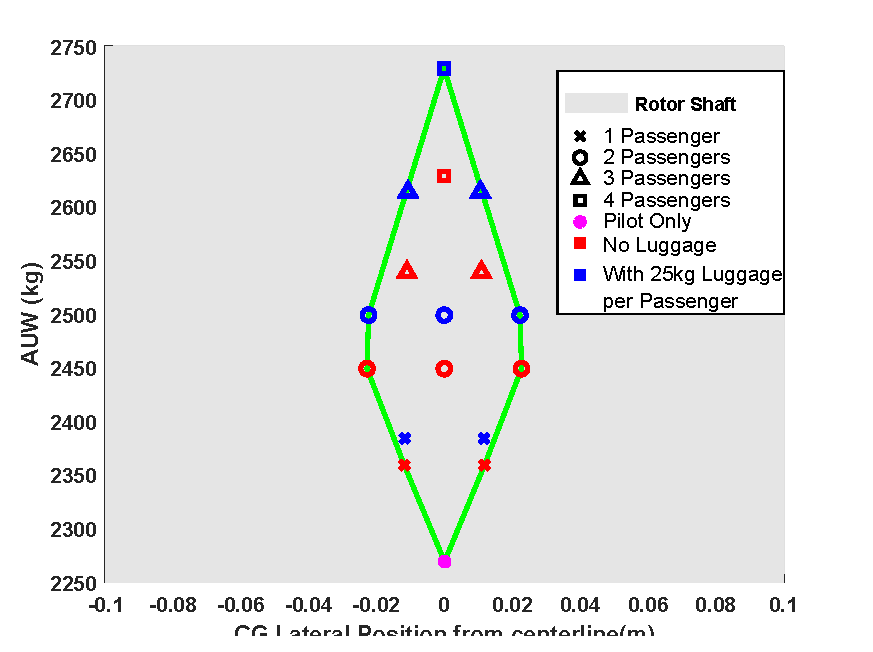
\includegraphics[width=\linewidth]{CGLATVAUW.eps}
  \captionof{figure}{Lateral ($y$-axis) CG against AUW}
  \label{fig:CGlat}
\end{minipage}%
\begin{minipage}{.49\textwidth}
  \centering
  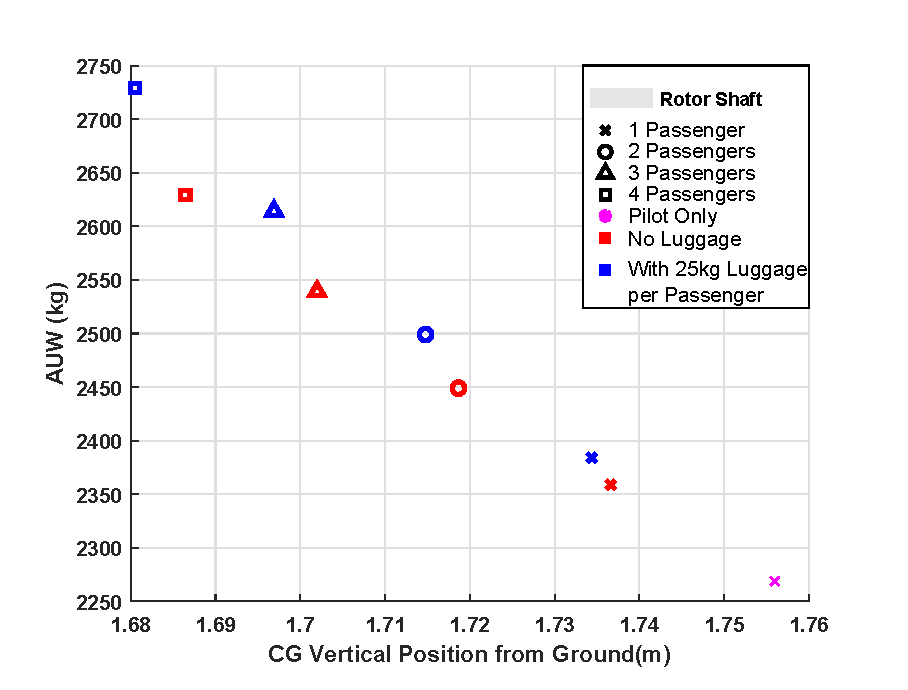
\includegraphics[width=\linewidth]{CGVERTVAUW.eps}
  \captionof{figure}{Vertical ($z$-axis) CG against AUW}
  \label{fig:CGvert}
\end{minipage}
\end{figure}

\begin{figure}[H]
    \centering
    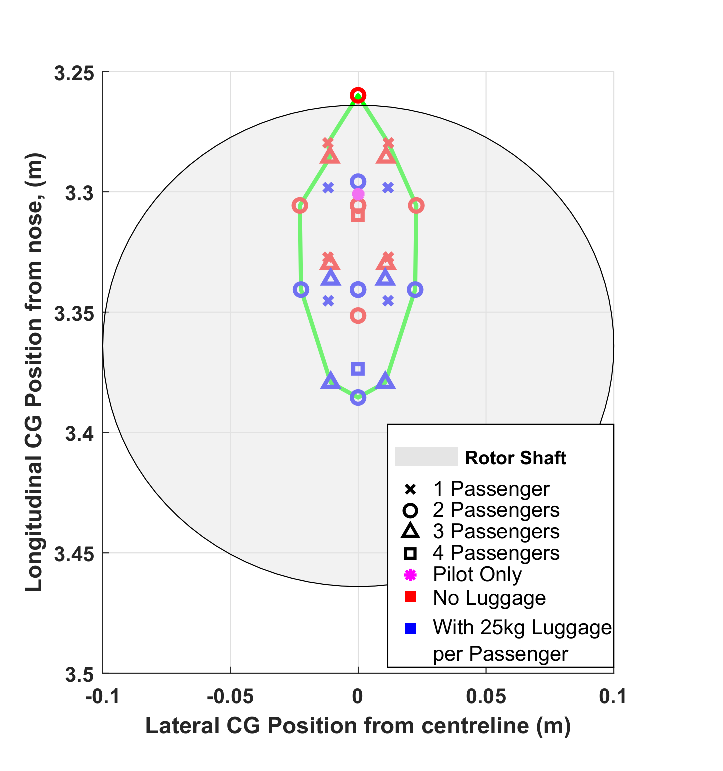
\includegraphics[width=0.4\textwidth]{CGLATVLONG.eps}
    \caption{Combined CG variation Longitudinal and Laterally axis}
    \label{fig:cglongvlat}
\end{figure}{}
%
% Appendix Moments of Inertia
%
\section{Moments of Inertia Equations}
\renewcommand\thefigure{B.\arabic{figure}}  
\setcounter{figure}{0}
\renewcommand\theequation{B.\arabic{equation}}  
\setcounter{equation}{0}
\renewcommand\thetable{B.\arabic{table}}  
\setcounter{table}{0}
\begin{align}
I_{xx}&=\sum_{i=1}^{n} m_{i}\left(\left(y_{i}-y_{C G}\right)^{2}+\left(z_{i}-z_{C G}\right)^{2}\right)\label{eq:ixx}\\
   I_{YY}&=\sum_{i=1}^{n} m_{i}\left(\left(x_{i}-x_{C G}\right)^{2}+\left(z_{i}-z_{C G}\right)^{2}\right)\\
   I_{ZZ}&=\sum_{i=1}^{n} m_{i}\left(\left(x_{i}-x_{C G}\right)^{2}+\left(y_{i}-y_{C G}\right)^{2}\right) \label{eq:izz}
\end{align}{}

\thispagestyle{empty}
%
% Appendix Trim Equations
%
\section{Trim Equations}
\renewcommand\thefigure{C.\arabic{figure}}  
\setcounter{figure}{0}
\renewcommand\theequation{C.\arabic{equation}}  
\setcounter{equation}{0}
\renewcommand\thetable{C.\arabic{table}}  
\setcounter{table}{0}
\thispagestyle{empty}
Hover Trim Equations
\begin{align}
    a_{\mathrm{1s}}&=\frac{T\,\left(h_{r}\,\gamma-x_{\mathrm{cg}}+\frac{D_{\mathrm{fZ}}\,l_{f}}{\mathrm{mg}}+\frac{D_{\mathrm{hZ}}\,l_{t}}{\mathrm{mg}}\right)}{\frac{dM_m}{da_{1s}}+T\,h_{r}}\\
    T&=-\frac{\mathrm{mg}}{\frac{D_{\mathrm{fZ}}}{\mathrm{mg}}+\frac{D_{\mathrm{hZ}}}{\mathrm{mg}}-1}\\
    \theta_f&=-\frac{T*(\gamma + a_{1s})}{mg} \label{eq:trimeq}
\end{align}{}

Cruise Trim Equations
\begin{align}
    T&=\sqrt{{\left(D_{f}+H_{r}\right)}^2+{\left(L_{f}-\mathrm{mg}\right)}^2}\\
    a_{\mathrm{1s}}&=\frac{M_{f}+D_{f}\,h_{f}+D_{h}\,h_{h}+D_{v}\,h_{v}+H_{r}\,h_{r}-L_{f}\,l_{f}+L_{t}\,l_{t}-T\,x_{\mathrm{cg}}}{\frac{dM_m}{da_{1s}}+T\,h_{r}}\\
    \alpha_{tpp}&=-\frac{H_r+D_h+D_v+D_f}{mg+L_t-L_f}\\
    \theta_f&=\alpha_{tpp}-a_{1s}-\gamma\\
    D_h&=\frac{1}{2}\,\rho\,V^2\,S_h\,(C_{d_\alpha}\,(\theta_f+\phi_t))\\
    \phi_t&=\frac{L_t}{0.5\,\rho\,V^2\,S_h\,C_{l_\alpha}}-\theta_f
\end{align}{}
%
% Appendix Pitch and Flapping Angles
%
\section{Pitch and Flapping Angles at Cruise and Hover}
\renewcommand\thefigure{D.\arabic{figure}}  
\setcounter{figure}{0}
\renewcommand\theequation{D.\arabic{equation}}  
\setcounter{equation}{0}
\renewcommand\thetable{D.\arabic{table}}  
\setcounter{table}{0}
\begin{figure}[H]
\centering
\begin{minipage}{.49\textwidth}
  \centering
  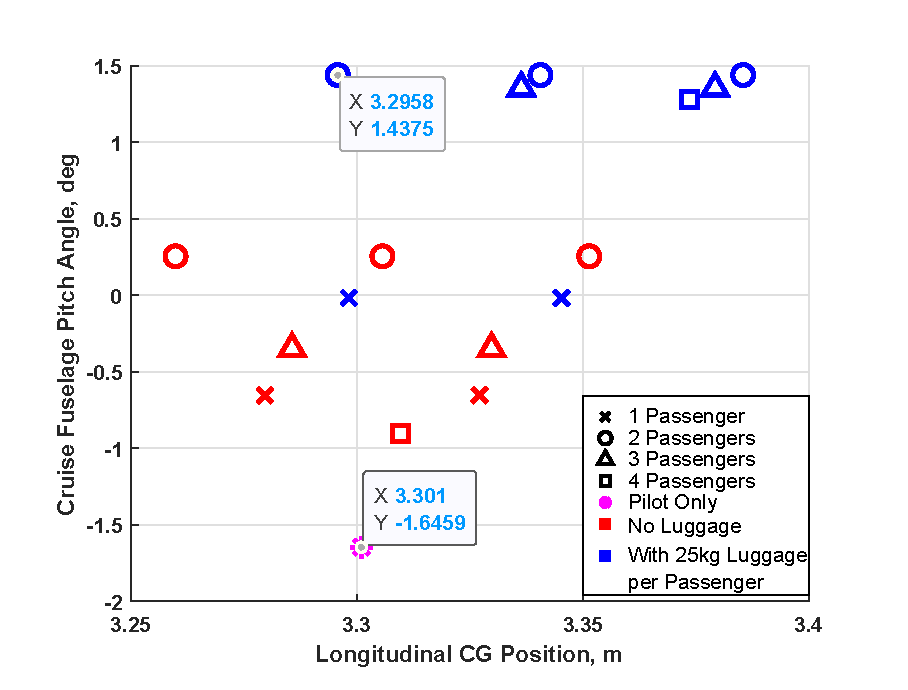
\includegraphics[width=\linewidth]{CGCRUISEP.eps}
  \captionof{figure}{Figure showing cruise pitch angles for each CG position for chosen design}
  \label{fig:CGCRUISEP}
\end{minipage}\hspace{0.2cm}
\begin{minipage}{.49\textwidth}
  \centering
  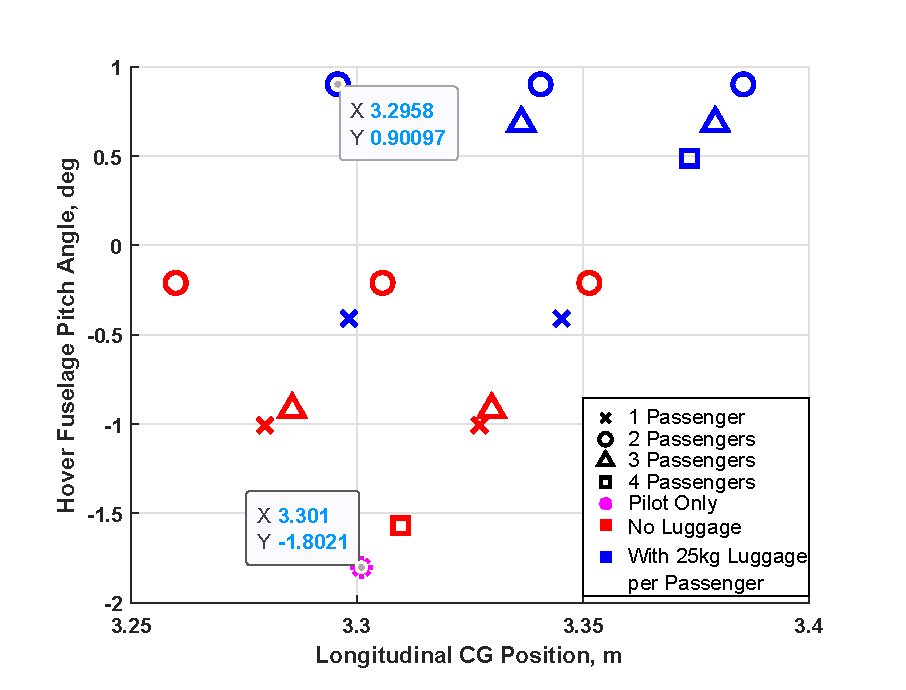
\includegraphics[width=\linewidth]{CGHOVERP.eps}
  \captionof{figure}{Figure showing hover pitch angles for each CG position for chosen design}
  \label{fig:CGHOVERP}
\end{minipage}
\end{figure}
\begin{figure}[H]
\centering
\begin{minipage}{.49\textwidth}
  \centering
  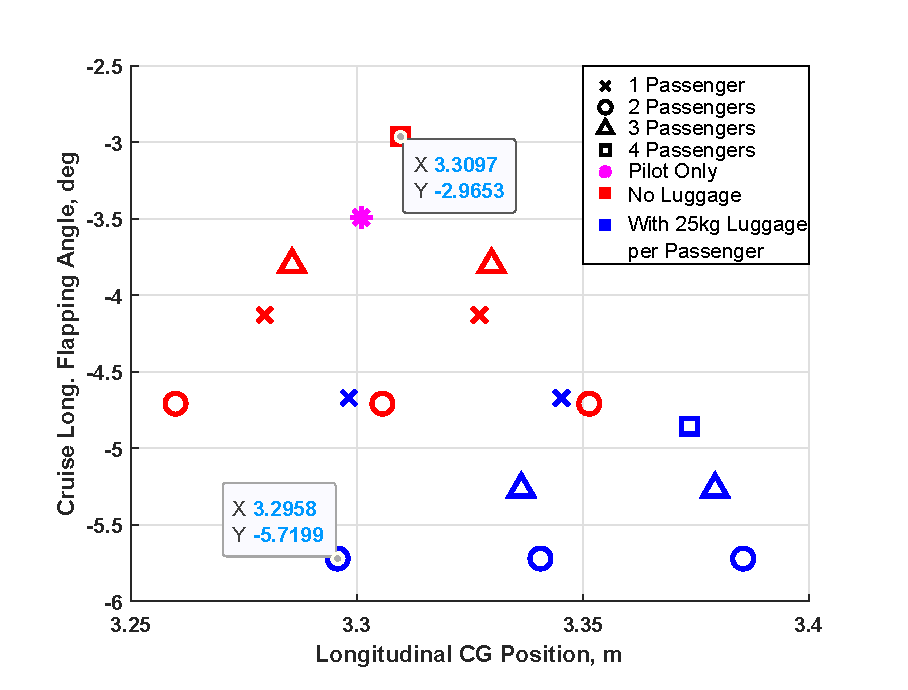
\includegraphics[width=\linewidth]{CGCRUISEF.eps}
  \captionof{figure}{Figure showing cruise flapping angles for each CG position for chosen design}
  \label{fig:CGCRUISEF}
\end{minipage}\hspace{0.2cm}
\begin{minipage}{.49\textwidth}
  \centering
  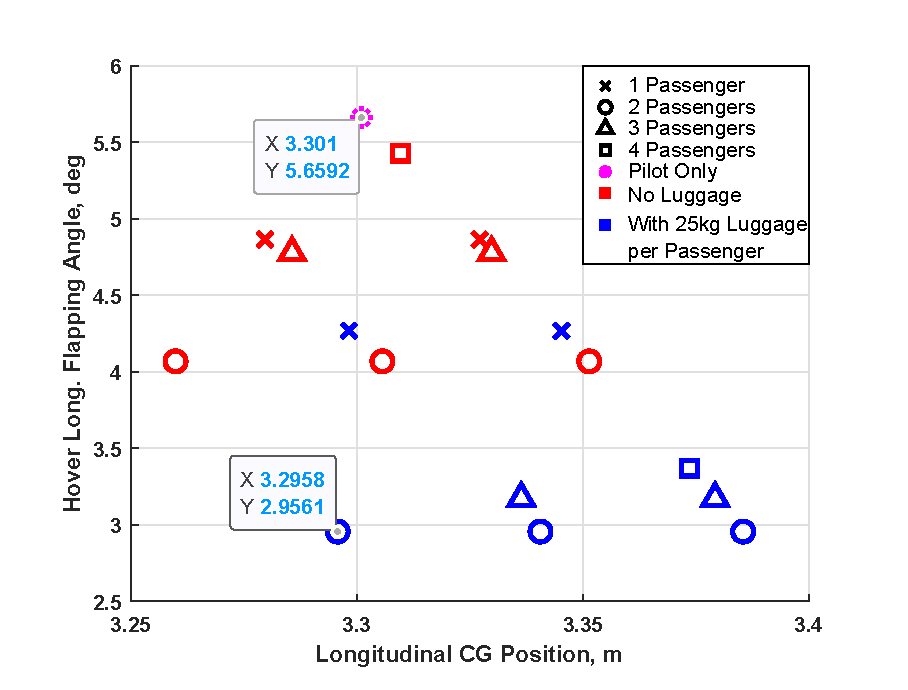
\includegraphics[width=\linewidth]{CGHOVERF.eps}
  \captionof{figure}{Figure showing hover flapping angles for each CG position for chosen design}
  \label{fig:CGHOVERF}
\end{minipage}
\end{figure}
\end{appendices}{}
\thispagestyle{empty}


\end{document}

%%NOTES
%Assumption  hover is in still air
%Cruise is in still air
%

%-------------------------------------------------------------------------------
% SNIPPETS
%-------------------------------------------------------------------------------

% \begin{figure}[!ht]
% 	\centering
% 	\includegraphics[width=0.8\textwidth]{file_name}
% 	\caption{}
% 	\centering
% 	\label{label:file_name}
% \end{figure}

%\begin{figure}[!ht]
%	\centering
%	\includegraphics[width=0.8\textwidth]{graph}
%	\caption{Blood pressure ranges and associated level of hypertension (American Heart Association, 2013).}
%	\centering
%	\label{label:graph}
%\end{figure}

%\begin{wrapfigure}{r}{0.30\textwidth}
%	\vspace{-40pt}
%	\begin{center}
%		\includegraphics[width=0.29\textwidth]{file_name}
%	\end{center}
%	\vspace{-20pt}
%	\caption{}
%	\label{label:file_name}
%\end{wrapfigure}

%\begin{wrapfigure}{r}{0.45\textwidth}
%	\begin{center}
%		\includegraphics[width=0.29\textwidth]{manometer}
%	\end{center}
%	\caption{Aneroid sphygmomanometer with stethoscope (Medicalexpo, 2012).}
%	\label{label:manometer}
%\end{wrapfigure}

%\begin{table}[!ht]\footnotesize
%	\centering
%	\begin{tabular}{cccccc}
%	\toprule
%	\multicolumn{2}{c} {Pearson's correlation test} & \multicolumn{4}{c} {Independent t-test} \\
%	\midrule	
%	\multicolumn{2}{c} {Gender} & \multicolumn{2}{c} {Activity level} & \multicolumn{2}{c} {Gender} \\
%	\midrule
%	Males & Females & 1st level & 6th level & Males & Females \\
%	\midrule
%	\multicolumn{2}{c} {BMI vs. SP} & \multicolumn{2}{c} {Systolic pressure} & \multicolumn{2}{c} {Systolic Pressure} \\
%	\multicolumn{2}{c} {BMI vs. DP} & \multicolumn{2}{c} {Diastolic pressure} & \multicolumn{2}{c} {Diastolic pressure} \\
%	\multicolumn{2}{c} {BMI vs. MAP} & \multicolumn{2}{c} {MAP} & \multicolumn{2}{c} {MAP} \\
%	\multicolumn{2}{c} {W:H ratio vs. SP} & \multicolumn{2}{c} {BMI} & \multicolumn{2}{c} {BMI} \\
%	\multicolumn{2}{c} {W:H ratio vs. DP} & \multicolumn{2}{c} {W:H ratio} & \multicolumn{2}{c} {W:H ratio} \\
%	\multicolumn{2}{c} {W:H ratio vs. MAP} & \multicolumn{2}{c} {\% Body fat} & \multicolumn{2}{c} {\% Body fat} \\
%	\multicolumn{2}{c} {} & \multicolumn{2}{c} {Height} & \multicolumn{2}{c} {Height} \\
%	\multicolumn{2}{c} {} & \multicolumn{2}{c} {Weight} & \multicolumn{2}{c} {Weight} \\
%	\multicolumn{2}{c} {} & \multicolumn{2}{c} {Heart rate} & \multicolumn{2}{c} {Heart rate} \\
%	\bottomrule
%	\end{tabular}
%	\caption{Parameters that were analysed and related statistical test performed for current study. BMI - body mass index; SP - systolic pressure; DP - diastolic pressure; MAP - mean arterial pressure; W:H ratio - waist to hip ratio.}
%	\label{label:tests}
%\end{table}
